\documentclass[11pt,a4paper]{jsarticle}
\usepackage[dvipdfmx]{graphicx}
\usepackage{url}

% --- ① タイトルと作成者情報 ---
\title{日本におけるデジタル化の状況}
\author{G684672026 鈴山 佐祐}
\date{2026年7月13日} % 提出する日付に合わせて適宜変更してください

\begin{document}

\maketitle

% --- ② 第1章 デジタル競争力ランキング ---
\section{デジタル競争力ランキング}
国際経営開発研究所(IMD)の調査\,\cite{imd}\,によると，日本のデジタル競争力のランキングは図\,\ref{fig:digital}\,に示すように，調査対象の64ヵ国中，総合で28位，準備分野で27位となっている．

\begin{figure}[htbp]
  \centering
  % ダウンロードしたグラフ画像「fig52.png」を読み込みます
  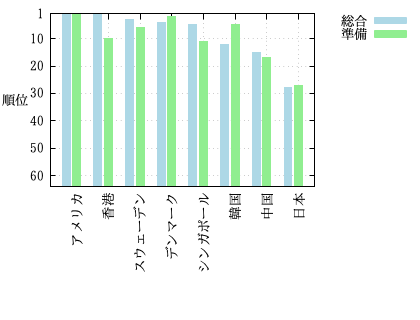
\includegraphics[width=0.7\linewidth]{fig52.png}
  \caption{デジタル競争力ランキング(64ヵ国中)}\label{fig:digital}
\end{figure}

% --- ③ 第2章 ブロードバンドの整備状況 ---
\section{ブロードバンドの整備状況}
OECDによるブロードバンド回線の普及に関する調査\,\cite{oecd}\,によると，表\,\ref{tab:broadband}\,に示すように，日本における100人あたりのモバイルブロードバンドの加入者数は190.5で，第1位になっている．2位はエストニアで，3位米国と続く．

\begin{table}[htbp]
  \caption{モバイルブロードバンドの加入者数(100人あたり)}\label{tab:broadband}
  \centering
  \begin{tabular}{|c|l|r|}
    \hline
    順位 & 国名 & 加入者数 \\ \hline
    1位 & 日本 & 190.5 \\ \hline
    2位 & エストニア & 179.9 \\ \hline
    3位 & 米国 & 169.0 \\ \hline
    4位 & フィンランド & 157.0 \\ \hline
    5位 & デンマーク & 141.7 \\ \hline
    6位 & ラトビア & 141.6 \\ \hline
    7位 & イスラエル & 139.9 \\ \hline
    8位 & オランダ & 133.7 \\ \hline
    9位 & ポーランド & 131.3 \\ \hline
    10位 & スウェーデン & 127.2 \\ \hline
  \end{tabular}
\end{table}

% --- ④ 第3章 考察 ---
\section{考察}
日本はモバイルブロードバンド加入者数が世界1位という良い環境があるのに、デジタル競争力ランキングでは28位と低いのが意外だった。
いくら通信インフラが整っていても、それを社会全体でうまく活かしきれていないのが原因ではないかと思う。
今後はこの優れたネットワーク環境を、ビジネスや行政の効率化にもっと役立てていくべきだと感じた。

% --- ⑤ 参考文献 ---
\begin{thebibliography}{9}
  \bibitem{imd} IMD.\quad IMD world digital competitiveness ranking.\quad \url{https://www.imd.org/centers/world-competitiveness-center/rankings/world-digital-competitiveness/}, 2021.
  \bibitem{oecd} OECD.\quad Broadband Portal.\quad \url{https://www.oecd.org/digital/broadband/broadband-statistics/}, 2022.
\end{thebibliography}

\end{document}